\chapter*{Заключение}
\addcontentsline{toc}{chapter}{Заключение}
\label{chapter:summary}

\section*{Списък с публикации}
\addcontentsline{toc}{section}{Списък с публикации}

\subsection*{Публикации в международни научни списания}
\addcontentsline{toc}{subsection}{Публикации в международни научни списания}

Предоставил съм списък с публикации, свързани с дисертацията. Изброените статии са публикувани без изключение в международни научни списания. [1] е ранна версия на въведението, както и на глава~\ref{chapter-openbiodiv} и съдържа труд по Задача 1 (Архитектура). Текстовете на публикациите [2, 3, 5, 6, 7] не са част от текста на дисертацията дословно, но съдържат труд по Задача 5 (Методи за работа). Представените в тези публикации идеи са в голяма степен включени в глава~\ref{chapter-case-study}, чиито гръбнак се формира от [4]; По този начин се постига Задача 5. [7] е публикувана в списанието ZooKeys с импакт-фактор 1.031 (към началото на 2018 г.). [8] е най-важната публикация в рамките на тази дисертация и е публикувана във реномиранато списание Journal of Biomedical Semantics с имакт-фактор 2.413 (към началото на 2018 г.). [8] съставлява съдържанието на глава~\ref{chapter-ontology} и е основната част от работата, изпълняваща Задача 2 (Онтология). Статията беше на заглавната страница на JBS в продължние на няколко месеца (фиг. \ref{fig:jbs-featured}). Глава~\ref{chapter-lod} и глава~\ref{chapter-rdf4r}, които формират Задачо 3, 4, се подготвят като ръкописи в международни списания. Освен това софтуерната библиотека RDF4R, описана в глава~\ref{chapter-rdf4r}, се подготвя да бъде изпратена в хранилището с отворен код rOpenSci\footnote{``We build software with a community of users and developers, and educate scientists about transparent research practices.'' \url{https://ropensci.org/}}.

Общият брой цитирания, които са натрупани, изключвайки авто-цитати е най-малко 19. Общият брой на натрупаните цитати, включително авто-цитати и цитати на работа извън обхвата на дисертацията, е най-малко 46 (Google Наука).

\begingroup
\newcounter{count}
\setcounter{count}{99}
\defcounter{maxnames}{\value{count}}%

\begin{enumerate}
\item \longfullcite{senderov_open_2016} (най-малко 3 уникални цитата)
\item \longfullcite{sarah_faulwetter_emodnet_2016}
\item \longfullcite{cardoso_species_2016} (най-малко 5 уникални цитата)
\item \longfullcite{senderov_online_2016} (най-малко 1 уникален цитат)
\item \longfullcite{penev_strategies_2017} (най-малко 6 уникални цитата)
\item \longfullcite{penev_arpha-biodiv:_2017} (най-малко 1 уникален цитат)
\item \longfullcite{arriaga-varela_review_2017} 
\item \longfullcite{senderov_openbiodiv-o:_2018} (най-малко 3 уникални цитата)
\end{enumerate}
\endgroup

\begin{figure}
\centering
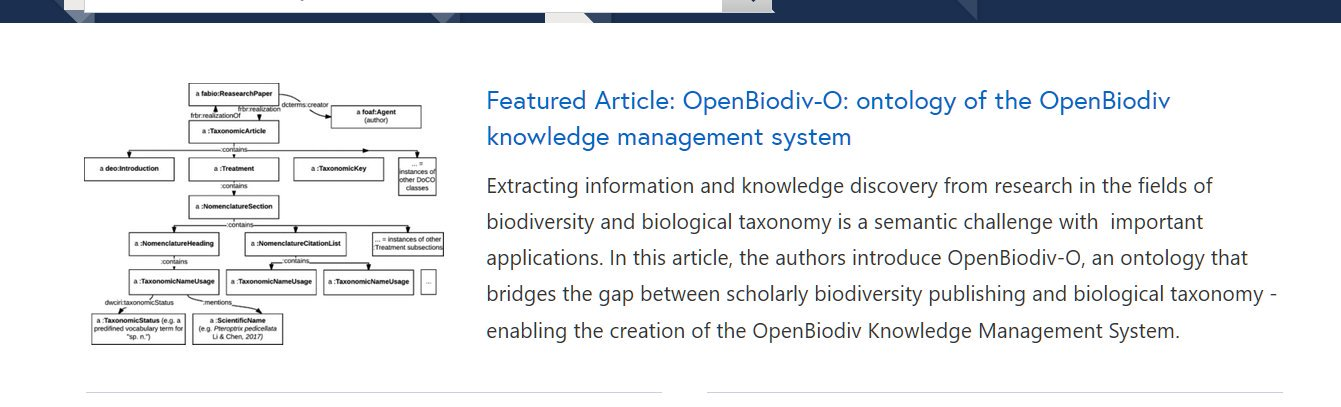
\includegraphics[width=\textwidth]{Figures/JBS-featured.jpg}
\decoRule
\caption{Статията относно OpenBiodiv-O е на началната страница на Journal of Biomedical Semantics.}
\label{fig:jbs-featured}
\end{figure}

\section*{Апробация на резултатите}
\addcontentsline{toc}{section}{Апробация на резултатите}

\subsection*{Доклади пред научен семинар на ПНЗ}
\addcontentsline{toc}{subsection}{Доклади пред научен семинар на ПНЗ}

\begin{enumerate}
    \item Доклад пред научен семинар на ИБЕИ на БАН на 26.10.2015 г. (“Публикуване, визуализация и разпространение на първични и геномни данни за биологичното разнообразие на основата на открита система за управление на информацията”).
    \item Доклад пред научен семинар в ИИКТ на БАН на 31.03.2016 г. (Open Biodiversity Knowledge Management System)
    \item Dоклад пред научен семинар на ИИКТ на БАН за 23.03.2018 г. (OpenBiodiv: a knowledge-based system of biodiversity information)
\end{enumerate}

\subsection*{Доклади пред научно мероприятие в чужбина или пред международно научно мероприятие у нас}
\addcontentsline{toc}{subsection}{Доклади пред научно мероприятие в чужбина или пред международно научно мероприятие у нас}

\begin{enumerate}
    \item Доклад пред международния симпозиум EU BON в София на 23.03.2016 г. (The Data Publishing Toolkit at EU BON: Automated creation of data papers, data and text integrated publishing via the ARPHA Publishing Platform.)
    \item Доклад по време на работната среща на BIG4 в Хавраники, Чехия на 03.06.2016 г. (Project Progress Report (OBKMS))
    \item Доклад по време на работната среща на BIG4 в Хавраники, Чехия на 03.06.2016 г. (Modern Methods of Systematic Research and the BOLD Algorithm)
    \item Уеб-базиран доклад (уебинар) пред международна аудитория в рамките на семинар на iDigBio на 16.07.2016 г. (Online direct import of specimen records from iDigBio instrastructure into taxonomic manuscripts)
    \item Доклад по време на работната среща на BIG4 в Копенхаген на 14.10.2016 г. (Midterm Progress Report)
    \item Доклад на международия симпозиум TDWG 2016 в Санта Клара де Сан Карлос от 5. до 9.12.2016 г. (Streamlining the Flow of Taxon Occurrence Data Between a Manuscript and Biological Databases)
    \item Доклад на международия симпозиум TDWG 2016 в Санта Клара де Сан Карлос от 5. до 9.12.2016 г. (The Open Biodiversity Knowledge Management System: A Semantic Suite Running on top of the Biodiversity Knowledge Graph)
    \item Доклад на международия симпозиум TDWG 2016 в Санта Клара де Сан Карлос от 5. до 9.12.2016 г. (Demonstrating the Prototype of the Open Biodiversity Knowledge Management System)
    \item Доклад на международия симпозиум TDWG 2016 в Санта Клара де Сан Карлос от 5. до 9.12.2016 г. (Creation of Data Paper Manuscripts from Ecological Metadata Language (EML))
    \item Уеб-базиран доклад пред междуродния семинар на работната група по семантични технология към Университета Вандербилт (Тенеси, САЩ) на 20.02.2017 г. (Open Biodiversity Knowledge Management System)
    \item Доклад на европейската конференция на биосистематиците, BioSyst.eu 2016 на 15.08.2017 г. (The OpenBiodiv Knowledge System: The Future of Access to Biodiversity Knowledge)
    \item Доклад на международия симпозиум TDWG 2017 в Отава, Канада от 1. до 6.10.2017 г. (OpenBiodiv Computer Demo: an Implementation of a Semantic System Running on top of the Biodiversity Knowledge Graph)
    \item Доклад на международия симпозиум TDWG 2017 в Отава, Канада от 1. до 6.10.2017 г. (OpenBiodiv: an Implementaion of a Semantic System Running on top of the Biodiversity Knowledge Graph)
    \item Постер на международия симпозиум TDWG 2017 в Отава, Канада от 1. до 6.10.2017 г. (OpenBiodiv: an Implementaion of a Semantic System Running on top of the Biodiversity Knowledge Graph)
    \item Доклад по време на работната среща на BIG4 в Ла Палма, Испания от 30. окт. до 3 ноем. 2017 г. (Midterm Progress Report)
    \item Доклад пред научен семинар на групата по биоинформатика (група Ронкуист) в Кралския природо-научен музей в Стокхолм на 29.11.2017 г.
\end{enumerate}

\section*{Основни научни и научно-приложни приноси}
\addcontentsline{toc}{section}{Основни научни и научно-приложни приноси}

В хода на изследването бяха постигнати всичките шест задачи и резултатите бяха публикувани в престижни международни списания и представени на големи конференции в България и в чужбина. Най-важните приноси на тезата са обобщени, както следва:

\paragraph{Принос 1.} Първият ключов принос на тезата е създаването на софтуерната архитектура на OpenBiodiv, очертана в глава~\ref{chapter-openbiodiv} и \cite{senderov_open_2016}. Този принос отговаря на Задача 1.

\paragraph{Принос 2.} Вторият ключов принос на дисертацията е създаването на домейн концептуализиране на публикуването на биоразнообразие и официална онтология OpenBiodiv-O, която дава възможност за свързване на знанията за биоразнообразието въз основа на научни публикации. OpenBiodiv-O служи за основа на свързаните отворени данни OpenBiodiv-LOD. Чрез разработването на онтология, насочена към биологичната таксономия, нашето намерение е да осигурим онтология, която запълва празнините между онтологиите за ресурсите на биологичното разнообразие като Дарвин-SW и онтологиите за семантично публикуване като онтологиите, съдържащи онтологиите на SPAR. Освен това считам, че е изгодно да се моделира самият таксономичен процес, а не някакво конкретно състояние на знанието. Този принос е описан в глава~\ref{chapter-ontology} и в \cite{senderov_openbiodiv-o:_2018} и изпълнява Задача 2. Неговият изходен код може да се види под \href{https://github.com/pensoft/openbiodiv-o}{github.com/pensoft/openbiodiv-o}.

\paragraph{Принос 3.} Третият ключов принос на дисертацията е създаването на свързани отворени данни, OpenBiodiv-LOD, състоящи се от трансформирани в RDF и интегрирани в база-данни твърдения за биоразнообразието. Твърденията са извлечени от XML на научни статии, публикувани от Пенсофт, XML таксономични дискусии, публикувани от Plazi, и CSV дъмп на таксономичната гръбнак на GBIF. OpenBiodiv-LOD е достъпен под \href{http://graph.openbiodiv.net}{\url{graph.openbiodiv.net}} и е описан в глава~\ref{chapter-lod}. Този принос отговаря на Задача 3.

\paragraph{Принос 4.} За да подпомогне създадаването на свързаните отворени данни, е разработен софтуерен пакет за средата за програмиране R, RDF4R. RDF4R дава възможност за манипулиране на RDF в R и улеснява за трансформирането на научни публикации от полуструктуриран XML формат в структуриран семантичен RDF. Този принос е обсъден в глава~\ref{chapter-rdf4r} и изпълнява Задача~4. Пакетът е достъпен онлайн като свободен софтуер под \href{http://github.com/pensoft/rdf4r}{github.com/pensoft/rdf4r}. Освен това допълнителен изходен код (неоптимизиран), описващ XML схемите на Пенсофт и Плаци и работещ в тандем с RDF4R за конвертиране на XML в RDF може да бъде намерен под \href{http://github.com/pensoft/ropenbio}{github.com/pensoft/ropenbio}.

\paragraph{Принос 5.} Механизмите за преобразуване на полуструктуриран XML в RDF се допълват от процеси за работа, които позволяват обогатяването на XML статии, публикувани от Пенсофт, чрез автоматично импортиране на данни от основните международни хранилища за данни за биологичното разнообразие: BOLD, GBIF, iDigBio , както и PlutoF. Освен това, благодарение на това дисертационно усилие е възможно автоматично да се създадат ръкописи от метаданни, кодирани в Ecological Metadata Language (EML). Обсъждането на тези автоматизирани работни процеси - автоматично генериране на data papers и автоматичен импорт на occurrence records - се извършва в глава~\ref{chapter-case-study}. Тя изпълнява Задача 5.

\paragraph{Принос 6.} За да допълним създаването на OpenBiodiv-LOD, ние разработихме уеб сайт който използва графа от знания \href{http://openbiodiv.net}{openbiodiv.net}, съдържащ семантична търсачка и приложения. Уебсайтът е обсъден в глава~\ref{chapter-webportal} и изпълнява Задача 6.

\section*{Декларация за оригиналност}
\addcontentsline{toc}{section}{Декларация за оригиналност}

Декларирам, че настоящата дисертация съдържа оригинални резултати, получени 
при проведени от мен научни изследвания, с подкрепата и съдействието на научния ми ръководител проф. Любомир Пенев и Издаделство Пенсофт, както и научния ми консултант доц. Кирил Симов и ИИКТ.  Резултатите,  които  са  получени,  описани  и/или  публикувани  от  други учени, са надлежно и подробно цитирани в библиографията.

Настоящата дисертация не е прилагана за придобиване на научна степен в друго 
висше училище, университет или научен институт.

Виктор Сендеров

